\Chapter{EXTRACTION DE TAXONOMIE EXPRESSIVE}
\label{chap:texp}


Dans le chapitre précédent, on a adopté un point de départ très restrictif pour extraire une taxonomie : une collection d'entités typées, représentées par leurs plongements vectoriels. On a essayé de reconstruire une information
% déjà trop spécifique ?
Le passage du graphe complet à ses plongements vectoriels entraîne nécessairement une perte d'information \hl{ref}.
En pratique, l'information contenue dans DBpédia est bien plus riche que cela; on peut donc se demander ce que l'on serait capable d'extraire si on s'autorisait l'accès à l'ensemble de DBpédia 
extraire des informations qui ne sont pas encore connues ?
Plus particulièrement, on a expliqué en introduction que manipuler des groupes d'instances plutôt que des concepts devait théoriquement permettre d'identifier de nouvelles classes. 

\section{Motivation et principes généraux}

Dans la section précédente, on a décrit une méthode pour extraire une hiérarchie entre les types à partir des seuls plongements d'entité. 

Méthode précédente : on s'interdit d'utiliser le linked data => comment retrouver l'information connue (la taxonomie DBpédia) à partir des seuls plongements vectoriels ?

Cette méthode : en utilisant toute l'information accessible, comment aller plus loin que ce qui existe (en l'occurence, trouver une taxonomie expressive – qui à l'heure actuelle n'existe pas)

Pas d'utilisation du Linked Data = méthode très descriptive, qui n'utilise pas toute l'information à notre disposition.

Schéma général proche de la méthode précédente: regroupement hiérarchique sur les entités, puis transformation de la hiérarchie entre entités en une hiérarchie sur les classes. Ici, étiquettage de la classe plus sophistiqué, puisuq'on s'autorise Linked Data.

Pourquoi ça marche ? Parce qu'on travaille sur un groupe d'entités dont on sait qu'elles sont sémantiquement proches, de par la géométrie de leurs plongements. Donc on restreint la dimension de l'espace de recherche, qui est un goulot d'étranglement habituel des méthodes d'extraction d'axiomes.

Toutefois, un ajout majeur : le retirage récursif des entités à regrouper pour limiter la propagation des erreurs dans l'arbre, limiter le bruit et affiner progressivement la spécificité des classes extraites.  % Plus un \textit{bag of tricks} pour que ça marche bien.

\paragraph{Remarque}

DBpédia, comme la plupart des graphes de connaissances, fonctionne sous l'hypothèse du monde ouvert : si un triplet est absent du graphe, cela ne signifie pas nécessairement qu'il est faux. Aussi, dans la suite, lorsqu'on écrit qu'une entité $x$ ne vérifie pas un prédicat logique $P$, cela doit être compris comme un raccourci pour écrire que l'assertion $P(x)$ n'est pas contenue dans le graphe, et non comme l'assertion $\neg P(x)$.

\paragraph{Notations}

On utilise les notations usuelles de la théorie des graphes : un graphe $G$ est représenté par une paire $(V, E)$ avec $V$ ses sommets, et $E \subseteq V \times V$ ses arêtes. En particulier, si $G$ est un arbre de clustering, l'arête $(C, C') \in E$ indique une relation d'inclusion $C \subset C'$; si $G$ est une taxonomie, l'arête $(A, B) \in E$ indique une subsumption $A \sqsubseteq B$. Par abus de notation, on notera parfois $x \in G$ plutôt que $x \in V$ pour indiquer qu'un élément est un sommet du graphe.

\section{Méthode proposée}

\begin{figure}[h]
    \centering
    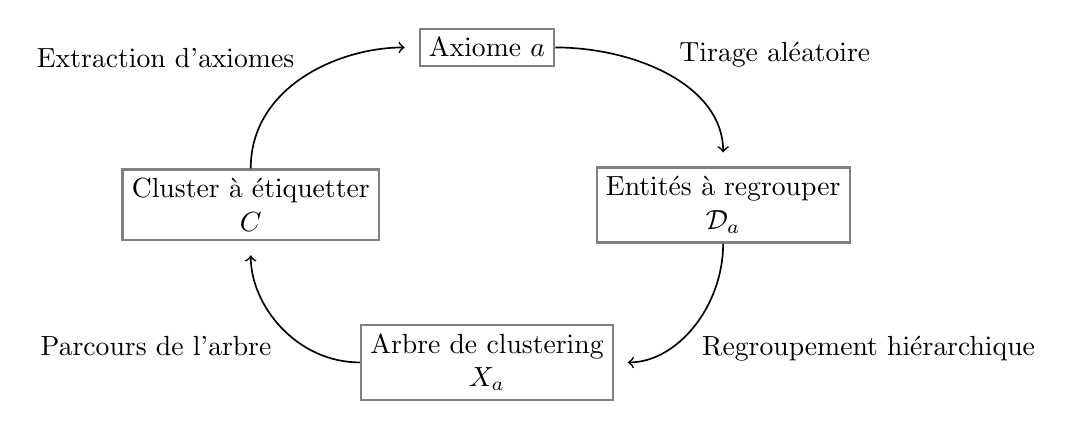
\begin{tikzpicture}[
  box/.style={draw=gray, thick, align=center},
  arrow/.style={->, semithick, shorten >=5pt,}
]
\def\l{2};
\node[box] (s2) at (1.5*\l, 0) {Entités à regrouper \\ $\mathcal{D}_a$};
\node[box] (s1) at (0, \l) {Axiome $a$};
\node[box] (s3) at (0, -\l) {Arbre de clustering \\$X_a$};
\node[box] (s4) at (-1.5*\l, 0) {Cluster à étiquetter \\$C$};

% \textit{Ensemble de $N$ entités vérifiant $a$}

\draw [arrow] (s1) to[out=0, in=90] node[auto] {Tirage aléatoire} (s2);
\draw [arrow] (s2) to[out=270, in=0] node[auto] {Regroupement hiérarchique} (s3);
\draw [arrow] (s3) to[out=180, in=270]  node[auto] {Parcours de l'arbre}  (s4);
\draw [arrow] (s4) to[out=90, in=180]  node[auto] {Extraction d'axiomes}  (s1);

\end{tikzpicture}
    \caption[Aperçu de la méthode d'extraction de taxonomie expressive]{Principe général de la méthode d'extraction de taxonomie : à partir d'un axiome initial $a$, on prélève aléatoirement des entités qui vérifient $a$, on les regroupe hiérarchiquement, et on parcours l'arbre obtenu pour extraire de nouveaux axiomes capables de décrire les clusters. On répète ces étapes pour construire progressivement une taxonomie complète du graphe; l'initialisation se fait avec $a = \top$.}
    \label{fig:texp-overview}
\end{figure}

La méthode d'extraction de taxonomie expressive commence par une phase de regroupement hiérarchique. Dans la méthode précédente, on avait comme seules données d'entrée un ensemble fixé d'entités typées $\cal{D}$. Ici au contraire, on s'autorise l'accès à tout le graphe, donc l'ensemble $\cal{D}$ sur lequel s'opère le regroupement hiérarchique est variable et change au cours de l'exécution de l'algorithme. À chaque étape $t$, on constitue un nouveau jeu de données $\mathcal{D}_t$.
On effectue alors un regroupement hiérarchique sur les plongements des entités de $\cal{D}_t$, puis on étiquette les clusters obtenus avec des axiomes logiques (l'extraction d'axiomes à partir de clusters est détaillée dans la section \ref{subsec:texp-exaxiom}). Chaque nouvel axiome extrait sert alors à créer un nouveau jeu de données $\mathcal{D}_{t+1}$, sur lequel on répète l'étape précédente, ce qui permet d'étendre itérativement la taxonomie prédite. L'algorithme \ref{algo:texp-main} présente les grandes étapes de cette méthode, et la figure \ref{fig:texp-overview} les résume.



\begin{algorithm}
\KwInput{un graphe de connaissance $\KG$}
\KwOutput{une taxonomie expressive $\Tpred$}
\Parameter{nombre d'entités à prélever à chaque étape $N_e$
%à compléter ?
}
\SetKwFunction{Preleve}{Preleve}
\SetKwFunction{Regroupe}{Regroupe}
\SetKwFunction{TrouveAxiomes}{EtiquetteArbre}
\SetKwFunction{Fusionne}{Fusionne}

\tcp{taxonomie construite récursivement :}
$\Tpred \leftarrow  (\{ \top \}, \varnothing)$ \;
\tcp{file d'axiomes à traiter :}
$\mathcal{AT} \leftarrow \{ \top \}$\;
% $t \leftarrow 0$ \;
% $\cal{C}_0 \leftarrow  \left\{ \{\bf{e}_1\}, \ldots, \{\bf{e}_N\} \right\}$\;
% $X = (\cal{C}_0, \emptyset)$ \;

\While{$\mathcal{AT}$ est non-vide}{
    $a \leftarrow $ premier axiome de la file $\mathcal{AT}$ \;
    \tcp{1 : prélevement/regroupement}
    $\mathcal{D}_a  \leftarrow$ \Preleve{$a, \KG, N_e$} \;
    $X_a \leftarrow$ \Regroupe{$\mathcal{D}_a$} \;
    \tcp{2 : extraction d'axiomes}
    $T_a \leftarrow$ \TrouveAxiomes{$X_a$} \;
    \For{chaque nouvel axiome $b$ de $T_a$}{
        ajouter $b$ à $\mathcal{AT}$ \;
    }
    $\Tpred \leftarrow $ \Fusionne{$\Tpred, T_a$} \;
    % $t \leftarrow t + 1$ \;
}
\Return{$X$}
\caption{Algorithme d'extraction de taxonomie expressive. Il consiste en deux étapes principales – l'une de prélevement et de regroupement d'entités, l'autre d'extraction d'axiomes – qui sont répétées de façon à construire récursivement la taxonomie $\Tpred$.}
\label{algo:texp-main}
\end{algorithm}



\subsection{Regroupement hiérarchique récursif avec retirage}



% Ensuite, pour chacun des axiomes $a_1, \ldots, a_k$ obtenus, on tire aléatoirement des entités qui vérifient cet axiome, ce qui donne de nouveaux ensembles d'entrées $\cal{D}_{t+1}, \ldots, \cal{D}_{t+k}$.


% Principe général
On dispose d'une file d'axiomes à traiter $\mathcal{AT}$, et de la taxonomie en cours de construction $\Tpred$. La file d'axiomes à traiter n'est autre que la liste des feuilles de $\Tpred$ qui n'ont pas encore été visitées. Lorsqu'on traite un axiome $\alpha$ de $\mathcal{AT}$, soit on parvient à extraire un sous-arbre $T_\alpha$ qui contienne des axiomes, et alors $T_\alpha$ est ajouté à $\Tpred$ à l'emplacement de $\alpha$, et les nœuds feuilles de $T_\alpha$ sont ajoutés à la file des axiomes à traiter; soit on ne trouve aucun sous-axiome pertinent pour $\alpha$, auquel cas $\alpha$ reste une feuille de $\Tpred$ et la recherche continue dans les autres axiomes de la file $\mathcal{AT}$, jusqu'à épuisement de $\mathcal{AT}$.

Pour la première étape, $\mathcal{AT}$ est initialisée à $\{\top\}$ : le seul axiome de $\mathcal{AT}$ est le concept universel $\top$ qui, par définition, est vérifié par toutes les entités du graphe. $\top$ sert de racine à la taxonomie, puisque c'est le seul axiome dont on soit sûr \textit{a priori} qu'il définisse toutes les entités.
La taxonomie $\Tpred$ est réduite à un seul sommet $\top$ et ne contient donc aucune arête. 

Tant que la file $\mathcal{AT}$ n'est pas vide, on retire son premier élément $a$, qui sert d'axiome d'entrée pour cette étape. On prélève aléatoirement, dans le graphe $\KG$, $N_e$ entités parmi celles qui vérifient $a$; cette étape correspond à la fonction \texttt{Preleve} de l'algorithme \ref{algo:texp-main}. Dans notre implémentation, le graphe est représenté grâce à une librairie Python spécifique, mais dans d'autres contextes, le langage de requête SPARQL pourrait être utilisé à cette fin. Les plongements de ces entités donne un nuage de points $\cal{D}_a$ de dimension $d \times N_e$, avec $d$ la dimension des plongements.

Sur ce nuage de point $\cal{D}_a$, on effectue un regroupement hiérarchique, similaire à celui décrit dans la section \ref{subsec:te-clustering}, qui correspond à la fonction \texttt{Regroupe} de l'algorithme \ref{algo:texp-main}.
Ici, on regroupe en utilisant comme mesure de similarité la distance cosinus, et comme critère de liaison le saut moyen. Autrement dit, on fusionne les clusters qui ont la plus faible distance cosinus moyenne entre leurs éléments. À l'étape $t$, notons $\cal{C}_t$ les clusters existants; les clusters $C_1$ et $C_2$ à fusionner sont choisis selon l'équation :
\begin{equation}
    C_1, C_2 = \argmin_{C_1, C_2 \in \cal{C}_t} \frac{1}{|C_1| \times |C_2|} \sum_{\bf{e_1}\in C_1} \sum_{\bf{e_2} \in C_2} d_\text{cos}(\bf{e_1, e_2})
\end{equation}

Le résultat est un arbre binaire, noté $X_a$, dont la racine est $\cal{D}_a$ tout entier, et dont les feuilles sont les $N_e$ éléments de $\cal{D}_a$. 

\subsection{Parcours et étiquettage de l'arbre}

Dans cette section, on se donne une fonction d'extraction d'axiome $\alpha$, telle que $\alpha(C)$ est un axiome logique qui qualifie le cluster $C$, si un tel axiome existe, et qui renvoie un symbole spécial \texttt{indéfini} dans le cas contraire. Un exemple d'une telle fonction est donné dans la section suivante. 

On effectue un parcours de l'arbre $X_a$, en excluant la racine $a$ qui est déjà étiquettée : pour un cluster $C$, on calcule $\alpha(C)$ pour trouver l'axiome associé à $C$. Si $\alpha(C) = \texttt{indéfini}$, le cluster $C$ n'a pas de signification logique accessible, et on poursuit la recherche dans les sous-clusters. Au contraire, si $\alpha(C)$ existe, on interrompt la recherche, et on ajoute $\alpha(C)$ à la file d'axiomes à visiter. Au-delà d'une certaine profondeur $D_\text{max}$ dans l'arbre, on arrête la recherche. On note $L_\alpha(a)$ l'ensemble des cluster $C$ étiquettés rencontrés lors de la recherche.


On construit alors la sous-taxonomie extraite $T_a$ à partir de $X_a$ : $T_a$ contient tous les axiomes extraits, c'est-à-dire les étiquettes de $X_a$, et sa structure reflète la structure entre les clusters, la subsumption entre axiomes correspondant à l'inclusion des clusters associés :
\begin{align}
    T_a = (& \{ \alpha(C) : C \in L_\alpha(a) \}, \nonumber \\
        & \{ (\alpha(C), \alpha(C')) : C, C' \in L_\alpha(a) \textrm{ et } C \subset C' \textrm{ et} \nonumber  \\
    & \forall D \in X_a, (C \subset D \subset C' \implies \alpha(D) = \texttt{indéfini})\})
\end{align}

Il s'agit du même principe que l'extraction de taxonomie de la méthode Hard Mapping présentée à l'équation \ref{eq:te-extract-tax-from-mapping} de la section \ref{ssubsec:te-hardmapping} : le parent d'un cluster étiquetté $C$ est le premier cluster étiquetté $C'$ qui contient $C$.


Enfin, si au moins l'une des feuilles de $X_a$ n'est pas couverte par un axiome $\alpha(C)$, c'est-à-dire s'il existe au moins une branche allant des feuilles à la racine qui ne contient pas d'étiquette, c'est qu'une partie de l'arbre n'a pas été décrite par un axiome, et qu'il reste potentiellement de nouveaux axiomes à extraire. Dans ce cas, un nœud spécial \texttt{<?>} est ajouté à $T_a$ et relié directement à $a$. La signification logique de ce nœud s'écrit :
\begin{equation}
    \texttt{<?>} = a \land \left( \bigwedge\limits_{C \in L_\alpha(a)} \neg \alpha(C) \right)
    \label{eq:texp-special-node}
\end{equation}
Soit, en langage courant, l'ensemble des éléments qui vérifient $a$ mais ne vérifient aucun des sous-axiomes $\alpha(C)$ de $a$. Cette définition purement négative n'est pas d'une grande utilité dans une taxonomie expressive, puisqu'elle exprime simplement la tautologie $C \lor \neg C = \top$. On utilise donc le symbole \texttt{<?>} pour signifier que la recherche n'est pas encore finie pour $a$ et qu'il reste des sous-axiomes de $a$ à trouver.

On donne un exemple de ce parcours à la figure \ref{fig:texp-stebbstep}. Dans cet exemple, l'axiome de départ $a$ est la classe \texttt{dbo:MeanOfTransportation}, et la profondeur maximale de recherche est fixée à $4$. L'arbre de clustering est parcouru en profondeur (figure \ref{subfig:texp-sbs1}), et trois sous-axiomes de $a$ sont extraits : \texttt{dbo:Automobile}, $\texttt{dbo:Ship} \lor \texttt{dbo:Aircraft}$ et $\exists \texttt{dbo:totalLaunches} . \texttt{integer}$. On peut voir que toutes les entités ne sont pas couvertes par un axiome : en effet, le cluster 6 n'est pas étiquetté. Cela signifie potentiellement que les trois axiomes extraits ne couvrent pas l'intégralité des instances de \texttt{dbo:MeanOfTransportation} et qu'il reste donc de nouveaux concepts à découvrir : on ajoute donc le nœud spécial \texttt{<?>} (figure \ref{subfig:texp-sbs2}).

\begin{figure}
    \centering
    \begin{subfigure}{\textwidth}
        \centering
        \begin{tikzpicture}[
  box/.style={draw=gray, thick, align=center},
  arrow/.style={->, shorten >=3pt, gray},
  node/.style={draw=gray, fill=gray!20},
  hnode/.style={draw=accent1, fill=accent1!20},
  snode/.style={draw=accent1, fill=accent1!20, very thick},
  exparr/.style={->, red, thick},
  axiomnode/.style={text=accent2},
  axiomedge/.style={dashed, accent2},
  short/.style={shorten >= 4pt, shorten <= 4pt}
]

\def\base{1.2};
\def\y{\base*1.3};
\def\dy{0.8};
\def\x{\base*1};
\def\sep{\base*0.3};
\def\xoff{\base*0.3};

\node [node] (a1) at (-4*\x-\sep, 0) {};
\node [node] (a2) at (-3*\x-\sep, 0) {};
\node [node] (a3) at (-2*\x, 0) {};
\node [node] (a4) at (-\x, 0) {};

\node (a5) at (\xoff, 0) {};
\node[snode] (a6) at (\xoff+\x, 0) {5};
\node[hnode] (a7) at (\xoff+2*\x, 0) {6};

\node [node] (b1) at (-3.5*\x-\sep, \y) {};
\node [node] (b2) at (-1.5*\x, \y) {};
\node [snode] (b3) at (\xoff, \y) {3};
\node [hnode] (b4) at (1.5*\x + \xoff, \y) {4};

\node [snode] (c1) at (-2.5*\x-0.5*\sep, \y*(1+\dy) {1};
\node [hnode] (c2) at (\xoff + 0.75*\x, \y*(1+\dy) {2};

\node [hnode] (root) at (0.5*\xoff-0.25*\sep-0.5*1.75*\x, \y+\y*\dy+\y*\dy*\dy) {0};

\draw[arrow] (b1) to (a1);
\draw[arrow] (b1) to (a2);
\draw[arrow] (b2) to (a3);
\draw[arrow] (b2) to (a4);

%\draw[arrow] (b3) to (a5);
\draw[arrow] (b4) to (a6);
\draw[arrow] (b4) to (a7);

\draw[arrow] (c1) to (b1);
\draw[arrow] (c1) to (b2);
\draw[arrow] (c2) to (b3);
\draw[arrow] (c2) to (b4);

\draw[arrow] (root) to (c1);
\draw[arrow] (root) to (c2);

\node[above left=0.1cm of root] (1a) {} ;
\node[above left=0.1cm of c1] (1b) {};
\draw[exparr, short] (1a) to 
%node[above left, red] {Recherche à gauche} 
(1b);

\node[right=0.4cm of c1] (2a) {};
\node[left=0.4cm of c2] (2b) {};
\draw[exparr] (2a) to[bend left] 
%node[below=0.4cm, red] {Recherche à droite} 
(2b);

\node[left=0.1cm of c2] (3a) {};
\node[above left=0.1cm of b3] (3b) {};
\draw[exparr] (3a) to (3b);

\node[right=0.1cm of b3] (4a) {};
\node[left=0.1cm of b4] (4b) {};
\draw[exparr] (4a) to[bend left] (4b) {};

\node[left=0.1cm of b4] (5a) {};
\node[above left=0.1cm of a6] (5b) {};
\draw[exparr] (5a) to (5b);

\node[right=0.01cm of a6] (6a) {};
\node[left=0.01cm of a7] (6b) {};
\draw[exparr] (6a) to[bend left] (6b) {};

\node[axiomnode, above right=1cm of c2] (lc2) {\texttt{indéfini}};
\node[axiomnode, above right=1cm of b4] (lb4) {\texttt{indéfini}};
\node[axiomnode, above right=1cm of a7] (la7) {\texttt{indéfini}};
\node[axiomnode, below right=1cm of a6] (la6) {$\exists \texttt{dbo:totalLaunches}.\texttt{integer}$};
\node[axiomnode, below left=1cm of a5, align=right] (la5) {$\texttt{dbo:Ship} \lor \texttt{dbo:Aircraft}$};
\node[axiomnode, above right=1cm of root] (lroot) {racine \texttt{dbo:MeanOfTransportation}};
\node[axiomnode, above left=1cm of c1] (lc1) {\texttt{dbo:Automobile}};

\draw[axiomedge] (c2) to (lc2);
\draw[axiomedge] (b4) to (lb4);
\draw[axiomedge] (a7) to (la7);
\draw[axiomedge] (a6.south) to (la6.west);
\draw[axiomedge] (b3.south) to (la5.east);
\draw[axiomedge] (c1) to (lc1.east);
\draw[axiomedge] (root) to (lroot.west);

\end{tikzpicture}
        \caption{Parcours du graphe $X_a$}
        \label{subfig:texp-sbs1}
    \end{subfigure}
    \begin{subfigure}{\textwidth}
        \centering
        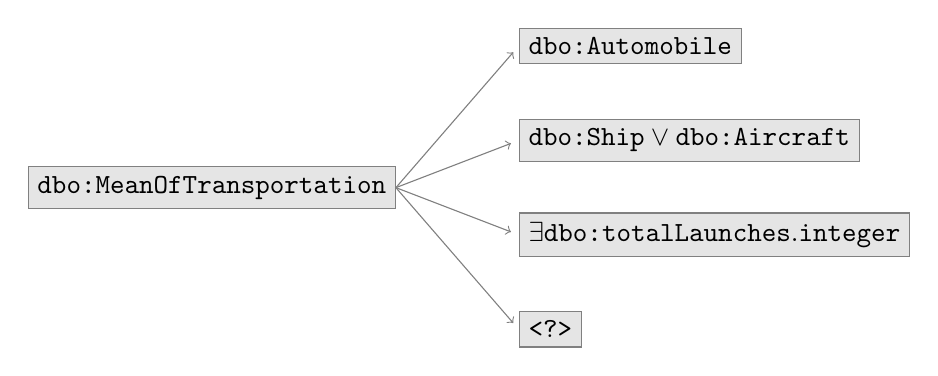
\begin{tikzpicture}[
  axiomnode/.style={fill=gray!20, draw=gray, anchor=west},
  axiomedge/.style={->, gray, shorten >=3pt},
]

\def\base{1.2};
\def\y{\base*1};
\def\x{\base*1.3};

\node[axiomnode] (a1) at (0, 3*\y) {\texttt{dbo:Automobile}};
\node[axiomnode] (a2) at (0, 2*\y) {$\texttt{dbo:Ship} \lor \texttt{dbo:Aircraft}$};
\node[axiomnode] (a3) at (0, \y) {$\exists \texttt{dbo:totalLaunches}.\texttt{integer}$};
\node[axiomnode] (a4) at (0, 0) {\texttt{<?>}};

\node[axiomnode, anchor=east] (root) at (-\x, 1.5*\y) {\texttt{dbo:MeanOfTransportation}};

\draw[axiomedge] (root.east) to (a1.west);
\draw[axiomedge] (root.east) to (a2.west);
\draw[axiomedge] (root.east) to (a3.west);
\draw[axiomedge] (root.east) to (a4.west);
\end{tikzpicture}
        \caption{Résultat obtenu $T_a$}
        \label{subfig:texp-sbs2}
    \end{subfigure}
    %\begin{tikzpicture}[
  box/.style={draw=gray, thick, align=center},
  arrow/.style={->, shorten >=3pt, gray},
  node/.style={draw=gray, fill=gray!20},
  hnode/.style={draw=accent1, fill=accent1!20},
  snode/.style={draw=accent1, fill=accent1!20, very thick},
  exparr/.style={->, red, thick},
  axiomnode/.style={text=accent2},
  axiomedge/.style={dashed, accent2},
  short/.style={shorten >= 4pt, shorten <= 4pt}
]

\def\base{1.2};
\def\y{\base*1.3};
\def\dy{0.8};
\def\x{\base*1};
\def\sep{\base*0.3};
\def\xoff{\base*0.3};

\node [node] (a1) at (-4*\x-\sep, 0) {};
\node [node] (a2) at (-3*\x-\sep, 0) {};
\node [node] (a3) at (-2*\x, 0) {};
\node [node] (a4) at (-\x, 0) {};

\node (a5) at (\xoff, 0) {};
\node[snode] (a6) at (\xoff+\x, 0) {5};
\node[hnode] (a7) at (\xoff+2*\x, 0) {6};

\node [node] (b1) at (-3.5*\x-\sep, \y) {};
\node [node] (b2) at (-1.5*\x, \y) {};
\node [snode] (b3) at (\xoff, \y) {3};
\node [hnode] (b4) at (1.5*\x + \xoff, \y) {4};

\node [snode] (c1) at (-2.5*\x-0.5*\sep, \y*(1+\dy) {1};
\node [hnode] (c2) at (\xoff + 0.75*\x, \y*(1+\dy) {2};

\node [hnode] (root) at (0.5*\xoff-0.25*\sep-0.5*1.75*\x, \y+\y*\dy+\y*\dy*\dy) {0};

\draw[arrow] (b1) to (a1);
\draw[arrow] (b1) to (a2);
\draw[arrow] (b2) to (a3);
\draw[arrow] (b2) to (a4);

%\draw[arrow] (b3) to (a5);
\draw[arrow] (b4) to (a6);
\draw[arrow] (b4) to (a7);

\draw[arrow] (c1) to (b1);
\draw[arrow] (c1) to (b2);
\draw[arrow] (c2) to (b3);
\draw[arrow] (c2) to (b4);

\draw[arrow] (root) to (c1);
\draw[arrow] (root) to (c2);

\node[above left=0.1cm of root] (1a) {} ;
\node[above left=0.1cm of c1] (1b) {};
\draw[exparr, short] (1a) to 
%node[above left, red] {Recherche à gauche} 
(1b);

\node[right=0.4cm of c1] (2a) {};
\node[left=0.4cm of c2] (2b) {};
\draw[exparr] (2a) to[bend left] 
%node[below=0.4cm, red] {Recherche à droite} 
(2b);

\node[left=0.1cm of c2] (3a) {};
\node[above left=0.1cm of b3] (3b) {};
\draw[exparr] (3a) to (3b);

\node[right=0.1cm of b3] (4a) {};
\node[left=0.1cm of b4] (4b) {};
\draw[exparr] (4a) to[bend left] (4b) {};

\node[left=0.1cm of b4] (5a) {};
\node[above left=0.1cm of a6] (5b) {};
\draw[exparr] (5a) to (5b);

\node[right=0.01cm of a6] (6a) {};
\node[left=0.01cm of a7] (6b) {};
\draw[exparr] (6a) to[bend left] (6b) {};

\node[axiomnode, above right=1cm of c2] (lc2) {\texttt{indéfini}};
\node[axiomnode, above right=1cm of b4] (lb4) {\texttt{indéfini}};
\node[axiomnode, above right=1cm of a7] (la7) {\texttt{indéfini}};
\node[axiomnode, below right=1cm of a6] (la6) {$\exists \texttt{dbo:totalLaunches}.\texttt{integer}$};
\node[axiomnode, below left=1cm of a5, align=right] (la5) {$\texttt{dbo:Ship} \lor \texttt{dbo:Aircraft}$};
\node[axiomnode, above right=1cm of root] (lroot) {racine \texttt{dbo:MeanOfTransportation}};
\node[axiomnode, above left=1cm of c1] (lc1) {\texttt{dbo:Automobile}};

\draw[axiomedge] (c2) to (lc2);
\draw[axiomedge] (b4) to (lb4);
\draw[axiomedge] (a7) to (la7);
\draw[axiomedge] (a6.south) to (la6.west);
\draw[axiomedge] (b3.south) to (la5.east);
\draw[axiomedge] (c1) to (lc1.east);
\draw[axiomedge] (root) to (lroot.west);

\end{tikzpicture}
    \caption{Un exemple d'étiquettage d'un arbre de clustering $X_a$, avec $a = \texttt{dbo:MeanOfTransportation}$. \textit{En haut}, chaque nœud représente un cluster de $X_a$; on représente en rouge les clusters qui sont visités au cours de l'extraction (les flèches rouges indiquent le parcours effectué, et le chiffre l'ordre de visite des clusters), et en gris ceux qui ne sont pas visités. En bleu, on représente l'axiome associé à chaque cluster visité; on indique par une bordure rouge épaisse les clusters qui sont effectivement étiquettés et qui apparaissent dans la taxonomie $T_a$. \textit{En bas}, on représente la taxonomie partielle obtenue $T_a$.}
    \label{fig:texp-stebbstep}
\end{figure}

%\begin{figure}
%    \centering
%    \begin{tikzpicture}[
  box/.style={draw=gray, thick, align=center},
  arrow/.style={->, shorten >=3pt},
  node/.style={draw=gray, fill=gray!20},
  hnode/.style={draw=accent1, fill=accent1!20},
  snode/.style={draw=accent1, fill=accent1!20, very thick}
]

\def\y{1.3};
\def\x{1};

\begin{scope}
\node[snode] (root) at (0, 1.8*\y) {$\top$};

\draw [->] (1, 1.8*\y) -- (3, 1.8*\y);
\end{scope}

\begin{scope}[xshift=4cm]

\node[node] (root) at (0, 1.8*\y) {$\top$};

\node[snode] (a) at (-\x, \y) {$A$};
\node[hnode] (b) at (\x, \y) {$B$};

\draw [arrow] (root) to (a);
\draw [arrow] (root) to (b);

\def\s{2};
\draw [->] (\s, 1.8*\y) -- (\s+2, 1.8*\y);
\end{scope}

\begin{scope}[xshift=10cm]

\node[node] (root) at (0, 1.8*\y) {$\top$};

\node[node] (a) at (-\x, \y) {$A$};
\node[snode] (b) at (\x, \y) {$B$};

\node[hnode] (a1) at (-2*\x, 0) {$A_1$};
\node[hnode] (a2) at (-\x, 0) {$A_2$};
\node[hnode] (a3) at (0, 0) {$A_3$};

\draw [arrow] (root) to (a);
\draw [arrow] (root) to (b);

\draw [arrow] (a) to (a1);
\draw [arrow] (a) to (a2);
\draw [arrow] (a) to (a3);

\end{scope}
\end{tikzpicture}
%    \caption[Principe de construction récursive d'une taxonomie]{Représentation de $\Tpred$ au cours des trois premières étapes de l'algorithme : à l'origne, $\Tpred$ est réduite au concept universel $\top$, puis deux sous-concepts $A$ et $B$ sont identifiés et rajoutés à $\Tpred$; c'est ensuite au tour de $A$ d'être exploré et ses sous-concepts $A_1, A_2, A_3$ sont ajoutés. On représente en rouge les axiomes non-encore explorés; la bordure épaisse représente le prochain axiome à explorer.}
%    \label{fig:texp-tree-expansion-old}
%\end{figure}


Si $T_a = (\varnothing, \varnothing)$, c'est-à-dire qu'aucun axiome n'a été trouvé en parcourant l'arbre $X_a$, alors $a$ n'aura pas de sous-axiome dans la taxonomie extraite et restera une feuille de $\Tpred$. Sinon, on remplace le nœud $a$ de $\Tpred$ par la sous-taxonomie $T_a$. Cette fusion de $\Tpred$ et $T_a$ correspond à la fonction \texttt{Fusionne} de l'algorithme \ref{algo:texp-main}, dont le code est décrit dans l'algorithme \ref{algo:texp-fusionne}. Une fois $\Tpred$ et $T_a$ fusionnées, on répète l'étape précédente, tant que la file d'axiomes $\mathcal{AT}$ n'est pas vide.

\paragraph{Extraction mono-niveau ou multi-niveaux}


Comme l'illustre la figure \ref{fig:texp-tree-expansion}, notre algorithme de parcours d'arbre peut fonctionner avec deux modes d'extraction : mono-niveau ou multi-niveaux. Dans le premier cas, dès qu'on identifie un axiome pour le cluster $C$, on interrompt la recherche dans les sous-clusters. La taxonomie $T_a$ extraite à partir de $X_a$ ne contient donc qu'un seule niveau, elle a donc pour sommets les axiomes extraits $\alpha(C_1), \ldots, \alpha(C_k)$ pour tous les $C_1, \ldots, C_k$ étiquettés, reliés directement à la racine $a$. La taxonomie $T_a$ s'écrit donc simplement :
\begin{equation}
    T_a = ( \{ \alpha(C) : C \in L_\alpha \}, \{ (\alpha(C), a) : C \in L_\alpha \} )
\end{equation}

\begin{figure}[h]
    \centering
    
    \begin{subfigure}{\textwidth}
        \centering
        \begin{tikzpicture}[
  box/.style={draw=gray, thick, align=center},
  arrow/.style={->, shorten >=3pt},
  node/.style={draw=gray, fill=gray!20},
  hnode/.style={draw=accent1, fill=accent1!20},
  snode/.style={draw=accent1, fill=accent1!20, very thick}
]

\def\y{1.3};
\def\x{1.2};

\begin{scope}
\node[snode] (root) at (0, 1.8*\y) {$\top$};

\draw [->] (1, 1.8*\y) -- (3, 1.8*\y);
\end{scope}

\begin{scope}[xshift=4cm]

\node[node] (root) at (0, 1.8*\y) {$\top$};

\node[snode, circle] (a) at (-\x, \y) {$A$};
\node[hnode, circle] (b) at (\x, \y) {$B$};

\draw [arrow] (root) to (a);
\draw [arrow] (root) to (b);

\def\s{2};
\draw [->] (\s, 1.8*\y) -- (\s+2, 1.8*\y);
\end{scope}

\begin{scope}[xshift=10cm]

\node[node] (root) at (0, 1.8*\y) {$\top$};

\node[node] (a) at (-\x, \y) {$A$};
\node[snode] (b) at (\x, \y) {$B$};

\node[hnode, circle] (a1) at (-2*\x, 0) {$A_1$};
\node[hnode, circle] (a2) at (-\x, 0) {$A_2$};
\node[hnode, circle] (a3) at (0, 0) {$A_3$};

\draw [arrow] (root) to (a);
\draw [arrow] (root) to (b);

\draw [arrow] (a) to (a1);
\draw [arrow] (a) to (a2);
\draw [arrow] (a) to (a3);

\end{scope}
\end{tikzpicture}
        \caption{Extraction mono-niveau}
        \label{subfig:tree-singlelevel}
    \end{subfigure}
    
    \begin{subfigure}{\textwidth}
        \centering
        \begin{tikzpicture}[
  box/.style={draw=gray, thick, align=center},
  arrow/.style={->, shorten >=3pt},
  node/.style={draw=gray, fill=gray!20},
  hnode/.style={draw=accent1, fill=accent1!20},
  snode/.style={draw=accent1, fill=accent1!20, very thick}
]

\def\y{1.3};
\def\x{1.2};
\begin{scope}
\node[snode] (root) at (0, 1.8*\y) {$\top$};

\draw [->] (1, 1.8*\y) -- (3, 1.8*\y);
\end{scope}

\begin{scope}[xshift=4cm]
\node[node] (root) at (0, 1.8*\y) {$\top$};

\node[node, circle] (a) at (-\x, \y) {$A$};
\node[node, circle] (b) at (\x, \y) {$B$};
\node[snode, circle] (a1) at (-2*\x, 0) {$A_1$};
\node[hnode, circle] (a2) at (-\x, 0) {$A_2$};
\node[node, circle] (a3) at (0, 0) {$A_3$};
\node[hnode, circle] (a31) at (-0.5*\x, -\y) {$A_{4}$};
\node[hnode, circle] (a32) at (0.5*\x, -\y) {$A_{5}$};
\node[hnode, circle] (b1) at (1.5*\x, 0) {$B_1$};

\draw [arrow] (root) to (a);
\draw [arrow] (root) to (b);

\draw [arrow] (a) to (a1);
\draw [arrow] (a) to (a2);
\draw [arrow] (a) to (a3);
\draw [arrow] (b) to (b1);

\draw[arrow] (a3) to (a31);
\draw[arrow] (a3) to (a32);


\def\s{2};
\draw [->] (\s, 1.8*\y) -- (\s+2, 1.8*\y);
\end{scope}

\begin{scope}[xshift=10cm]

\node[node] (root) at (0, 1.8*\y) {$\top$};

\node[node] (a) at (-\x, \y) {$A$};
\node[node] (b) at (\x, \y) {$B$};

\node[node] (a1) at (-2*\x, 0) {$A_1$};
\node[snode] (a2) at (-\x, 0) {$A_2$};
\node[node] (a3) at (0, 0) {$A_3$};
\node[hnode] (a31) at (-0.5*\x, -1*\y) {$A_{4}$};
\node[hnode] (a32) at (0.5*\x, -1*\y) {$A_{5}$};
\node[hnode] (b1) at (1.5*\x, 0) {$B_1$};

\node[node, circle] (a11) at (-2*\x, -1*\y) {$A_{6}$};
\node[hnode, circle] (a111) at (-2.8*\x, -2*\y) {$A_{7}$};
\node[hnode, circle] (a112) at (-1.2*\x, -2*\y) {$A_{8}$};

\draw [arrow] (root) to (a);
\draw [arrow] (root) to (b);

\draw [arrow] (a) to (a1);
\draw [arrow] (a) to (a2);
\draw [arrow] (a) to (a3);
\draw [arrow] (b) to (b1);

\draw[arrow] (a3) to (a31);
\draw[arrow] (a3) to (a32);

\draw[arrow] (a1) to (a11);
\draw[arrow] (a11) to (a111);
\draw[arrow] (a11) to (a112);


\end{scope}
\end{tikzpicture}
        \caption{Extraction multi-niveaux}
        \label{subfig:tree-multilevel}
    \end{subfigure}
    
    \caption[Extraction mono-niveau et extraction multi-niveaux]{Représentation de $\Tpred$ au cours des trois premières étapes de l'algorithme, pour une extraction mono-niveau (\textit{en haut}) et une extraction multi-niveaux (\textit{en bas}). Dans les deux cas, $\Tpred$ est réduite au concept universel $\top$ lors de l'initialisation. Dans le premier cas, on ajoute un unique niveau à chaque étape; dans le second, on s'autorise à en ajouter plusieurs. On représente en rouge les axiomes non-encore explorés, qui appartiennnent donc à la file d'axiomes non-traités $A$; la bordure épaisse représente le prochain axiome à explorer; les cercles indiquent les axiomes qui viennent d'être extraits.}
    \label{fig:texp-tree-expansion}
\end{figure}


Ainsi, dans la figure \ref{subfig:tree-singlelevel}, on extrait $A \sqsubset \top$ et $B \sqsubset \top$ à l'étape une, puis $A_1 \sqsubset A$, $A_2 \sqsubset A$, $A_3 \sqsubset A$ à l'étape deux.

À l'inverse, dans le cas multi-niveaux, on poursuit la recherche dans les sous-clusters de $C$, même quand $C$ est étiquetté, et ce, jusqu'à atteindre la profondeur maximale $D$. La taxonomie $T_a$ a donc potentiellement plusieurs niveaux. Cette approche est illustrée à la figure \ref{subfig:tree-multilevel} : trois niveaux sont extraits lors de la première étape, et deux autres lors de la seconde. À chaque étape, seules les feuilles de $T_a$ sont ajoutées à la file d'axiomes $\mathcal{AT}$.




L'approche multi-niveaux permet de réduire le nombre d'étapes de plongement-regroupement nécessaires – et donc potentiellement diminuer la durée d'extraction totale, tout en tirant au maximum parti de la structure d'arbre de $X_a$. À l'inverse, dans le cas mono-niveau, la structure d'arbre sert principalement à déterminer dynamiquement le nombre de clusters pertinents. Dans nos essais, on utilisera uniquement la méthode mono-niveau (quitte à exécuter un plus grand nombre d'étapes), car elle est moins sensible aux changements de paramètres et paraît globalement plus robuste. L'algorithme \ref{algo:texp-trouve} contient le pseudo-code de cette approche.

\begin{algorithm}
\SetKwFunction{Etiq}{EtiquetteArbre}
\SetKwData{NT}{NonVisités}
\SetKwData{root}{racine}
\SetKwData{indef}{indéfini}
\SetKwData{addspe}{ajouteNoeudSpecial}
\SetKwFunction{TrouveAxiomes}{TrouveAxiomes}

\KwInput{un arbre de clustering $X_a$}
\KwOutput{une taxonomie partielle $T_a$}
\Parameter{profondeur maximale du parcours $D$}
\SetKwProg{Fn}{Fonction}{:}{}
\Fn{\Etiq{$X_a$}}{
    \root $\leftarrow$ racine de $X_a$ \;
    \NT $\leftarrow \{$ sous-clusters de \root $\}$ \;
    $L_\alpha \leftarrow \varnothing$ \;
    \addspe $\leftarrow \texttt{Faux}$ \; 
    \While{\NT n'est pas vide}{
        $C \leftarrow $ premier élément de \NT \;
        $\alpha(C) \leftarrow $ \TrouveAxiomes{$C, \delta$} \;
        \eIf{$\alpha(C)$ n'est pas \indef}{
            ajouter $C$ à $L_\alpha$ \;
        }{
            \eIf{la profondeur de $C$ est inférieure à $D$}{
                ajouter les sous-clusters de $C$ à \NT \;
            }{
                $\addspe \leftarrow \texttt{Vrai}$ \;
            }
        }
    }
    $V_a \leftarrow \{ \alpha(C) \}_{C \in L_\alpha}$ \;
    $E_a \leftarrow \{ (\alpha(C), \root) : C \in L_\alpha \}$ \;
    \If{\addspe est vrai}{
        ajouter \texttt{<?>} à $V_a$\;
        ajouter $(\texttt{<?>}, \root)$ à $E_a$ \; 
    }
    $T_a \leftarrow (V_a, E_a)$ \;
    \Return{$T_a$}
}
\caption{Pseudo-code pour la fonction \texttt{EtiquetteArbre} de l'algorithme \ref{algo:texp-main}. Cette fonction parcourt l'arbre de clustering $X_a$ et cherche à étiquetter les clusters avec des axiomes, et renvoie une taxonomie partielle sur ces axiomes. La fonction \texttt{TrouveAxiomes} est décrite dans la section \ref{subsec:texp-exaxiom}.}
\label{algo:texp-trouve}
\end{algorithm}

\paragraph{Le cas des nœuds spéciaux \texttt{<?>}} Dans l'étape précédente, le cas où l'axiome de départ $a$ est l'axiome spécial \texttt{<?>} est traité un peu différemment du cas général. Les données d'entrées sont toujours tirées aléatoirement, suivant la formule \ref{eq:texp-special-node}; le regroupement hiérarchique et l'extraction de la sous-taxonomie $T_a$ suit une procédure identique. Ensuite, on rattache $T_a$ à $\Tpred$. La taxonomie $\Tpred$ en cours d'extraction contient alors toujours le nœud spécial \texttt{<?>}, qu'on ne souhaite pas garder : on modifie alors $\Tpred$ en rattachant directement les successeurs directs de \texttt{<?>} avec le prédecesseur direct de \texttt{<?>}, on ré-écrit donc les chemins $\alpha \rightarrow \texttt{<?>} \rightarrow \beta$ en $\alpha \rightarrow \beta$, et on supprime \texttt{<?>} de $\Tpred$.

\begin{algorithm}
\SetKwFunction{Fusionne}{Fusionne}
\SetKwProg{Fn}{Fonction}{:}{}
\Fn{\Fusionne{$T_1, T_2$}}{
    $a \leftarrow$ axiome racine de $T_2$ \;
    $(V_1, E_1) \leftarrow T_1$ \;
    $(V_2, E_2) \leftarrow T_2$ \;
    $V \leftarrow V_1 \cup V_2$ \;
    $E \leftarrow E_1 \cup E_2$ \;
    \If{$a$ est de la forme \texttt{<?>}}{
        \For{$\alpha, \beta \in V$ tels que $\alpha \rightarrow a \rightarrow \beta$}{
            \tcp{on relie directement beta à alpha}
            $E \leftarrow \left(E \setminus \{(\beta, a), (a , \alpha) \}\right) \cup \{ (\beta, \alpha) \} $ \;
        }
        $V \leftarrow V \setminus \{ a \}$ \;
    }
    $T \leftarrow (V, E)$ \;
    \Return{$T$}
}
\caption{Pseudo-code pour la fonction \texttt{Fusionne} de l'algorithme \ref{algo:texp-main}. Cette fonction ajoute la taxonomie $T_2$ à la taxonomie $T_1$, en traitant éventuellement le cas où $a$ (l'axiome qui a servi à construire $T_2$) est un nœud spécial \texttt{<?>}.}
\label{algo:texp-fusionne}
\end{algorithm}




% \begin{figure}
%     \centering
%     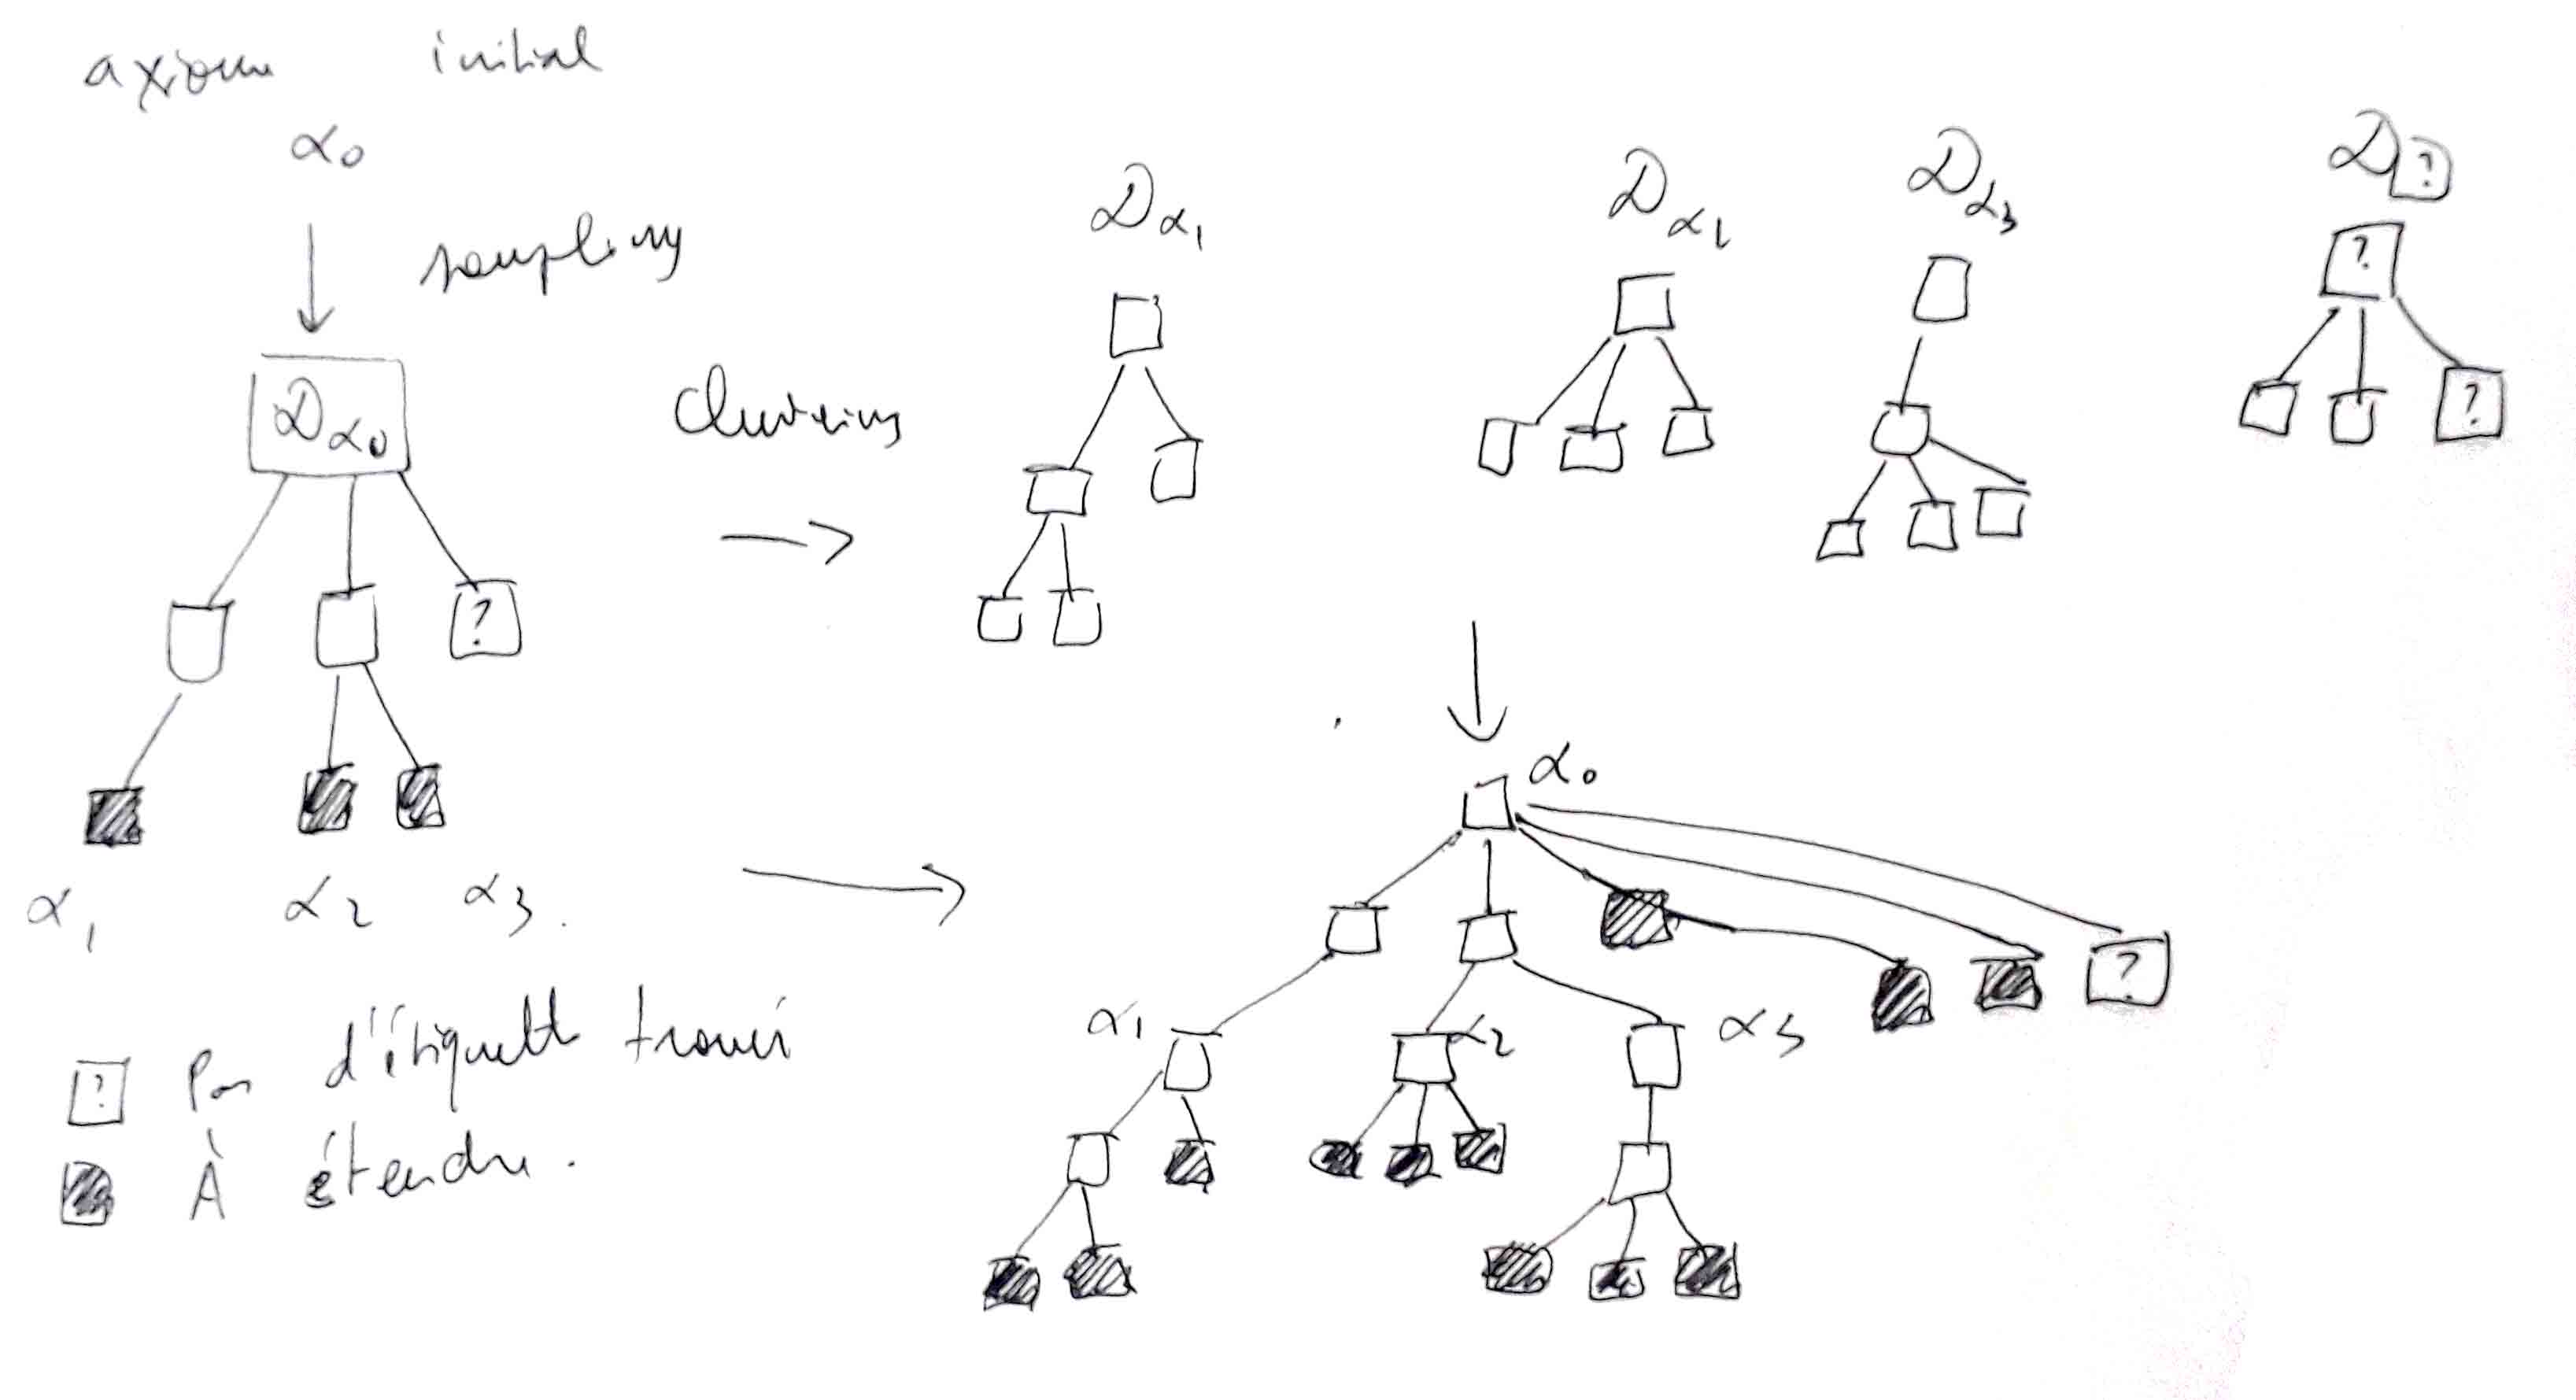
\includegraphics[width=\textwidth]{img/expressive_extraction_overview.jpg}
%     \caption[Principe de l'expansion d'arbre taxonomique]{(Provisoire) Principe général pour % l'expansion d'arbres. À partir d'un axiome initial $\alpha_0$, un arbre est construit, et % trois nouveaux axiomes $\alpha_1, \alpha_2, \alpha_3$. Trois nouveaux arbres sont % construits, et ajoutés à l'arbre initial. Le procédé est répété, jusqu'à obtenir une % taxonomie expressive complète.}
%     \label{fig:my_label}
% \end{figure}


\paragraph{Seuil adaptatif} On expérimente également une variante de l'algorithme précédent, dans laquelle le seuil $\delta$ pour l'extraction d'axiome varie au cours du temps : au début, le seuil de validité des axiomes est fixé à une valeur initiale élevée $\delta = \delta_\text{init}$; puis, à chaque fois que la file d'axiome $A$ est vidée, on diminue $\delta$ d'une quantité $d\delta$, on ré-initialise $A = \{ \top \}$, et on recommence l'algorithme, jusqu'à atteindre un seuil minimal $\delta_\text{min}$ . Des valeurs typiques sont $\delta_\text{init} = 0.9, d\delta = 0.1, \delta_\text{min} = 0.5$.

Partir avec un seuil bas dès le début ne permet pas de discriminer efficacement les axiomes valides des axiomes invalides; à l'inverse, conserver un seuil élevé tout au long de l'algorithme conduit à écarter des axiomes valides : en effet, les graphes de connaissance étant incomplets et bruités – certaines relations manquent, des triplets peuvent être erronés etc., un axiome valide peut être imparfaitement vérifié. La technique du seuil adaptatif permet de contourner en partie cette limitation, en imposant d'abord un seuil haut qui permet de créer une ossature fiable pour la taxonomie, puis en relâchant ce seuil pour aggréger de nouveaux axiomes plus incertains.



% Rappeler le principe général
% 
% Exposer le principe de récursivité avec un schéma
% 
% Modalités de retirage
% 
% Expérimentation avec/sans retirage
% 
% Seuil adaptatif


\subsection{Extraction d'axiomes}
\label{subsec:texp-exaxiom}

L'étape de regroupement hiérarchique décrite précédemment suppose l'existence d'une méthode pour étiquetter automatiquement un cluser avec un axiome logique. Cette méthode doit estimer si un cluster correspond à un échellon pertinent, et, le cas échéant, lui attribuer un axiome logique capable de décrire les entités contenues dans ce cluster. Si le cluster n'est pas jugé pertinent, la méthode doit renvoyer \texttt{indéfini}.

La recherche d'un axiome $A$ pour un cluster $C$ ne peut pas se baser uniquement sur les entités du cluster $C$ : en effet, on cherche un axiome qui qualifie $C$ et \textit{uniquement} $C$. On doit donc s'assurer que les entités qui ne font pas partie de $C$ ne vérifient pas $A$, ce qui implique de disposer d'un ensemble d'exemples négatifs, en plus des exemples positifs que sont les entités de $C$. Un axiome doit ainsi remplir deux conditions : \textbf{couverture} (l'axiome est vérifié par la majorité des éléments du cluster) et \textbf{spécificité} (l'axiome n'est pas ou peu vérifié hors du cluster). 
% Pour satisfaire ces deux conditions, on doit disposer d'exemples positifs (les entités contenues dans le cluster, pour vérifier la couverture) et d'exemples négatifs (des entités non contenues dans le cluster, pour vérifier la spécificité). 

Toutefois, si l'on choisit comme exemples négatifs l'ensemble des entités qui ne sont pas dans $C$, on doit à nouveau considérer l'intégralité du graphe; on perd donc l'intérêt d'avoir réduit l'espace de recherche grâce au tirage aléatoire et au regroupement, et on retrouve la difficulté inhérente à l'extraction d'axiomes dans un graphe de grande taille.
On pourrait choisir de tirer aléatoirement des exemples négatifs, mais on risque alors de diminuer la spécificité des axiomes extraits. Par exemple, supposons que l'on cherche à étiquetter un sous-cluster de \texttt{dbo:Writer} : on souhaitera alors extraire des axiomes précis, capables par exemple de distinguer les poètes des romanciers ou des dramaturges. Pourtant, si on compare les entités d'un tel sous-cluster à des entités quelconques du graphe, il est probable qu'un simple axiome $\exists \texttt{dbo:isWriterOf}.\top$ suffise à obtenir une très bonne spécificité. Les exemples négatifs doivent donc être de plus en plus proches des exemples positifs à mesure que l'on s'enfonce dans la taxonomie.


Or, l'arbre de clustering fournit justement, pour chaque cluster $C$, un groupe d'entités proche mais disjoint de $C$ : il s'agit du cluster \textit{voisin}. L'arbre étant binaire, chaque cluster (hors clusters feuilles) est partitionné en deux sous-clusters; ces deux sous-clusters sont dits \textit{voisins} l'un de l'autre. Deux clusters voisins ont le même cluster parent, ce qui indique une proximité entre eux; ils sont disjoints l'un de l'autre, ce qui peut indiquer une différence entre leurs entités. Notre approche consiste donc à expliquer, au moyen d'un axiome logique, la division d'un cluster parent en deux sous-clusters. 
La méthode d'extraction choisie est simple, et se base sur des statistiques d'occurrence au sein d'un cluster, dans la lignée de la méthode SSI présentée dans la section \ref{subsec:litt-te-graph}. % Les points cruciaux de notre approche ne reposent pas tant sur cette extraction proprement dite, que s
Toutefois, d'autres algorithmes d'extraction d'axiomes pourraient être utilisés. 

Dans les paragraphes qui suivent, on formalise les notions de couverture et de spécificité esquissées ici, et on présente le cadre de notre méthode d'extraction et son fonctionnement.

\subsubsection{Couverture, spécificité et score de partition}
Soit $C = \{e_1, e_2, \ldots, e_n \} \subseteq \Ent$ un cluster contenant $n$ entités. Si $C$ n'est pas une feuille, alors il a deux sous-clusters gauche et droit, notés $L$ et $R$, et contenant respectivement $n_1$ et $n_2$ entités, avec $n = n_1 + n_2$. En notant $\sqcup$ l'union disjointe, on a donc :
\begin{equation}
C = L \sqcup R
\end{equation}
Pour un axiome logique $A$ et une entité $x \in \Ent$, on note $A(x)$ si $x$ vérifie l'axiome $A$. On se propose d'expliquer la séparation du cluster $C$ en ses deux sous-clusters, c'est-à-dire d'identifier des axiomes qui sont vrais dans $L$ mais pas dans $R$. Si on trouve un tel axiome, on pourra alors l'utiliser comme étiquette pour le cluster $L$. Si on n'en trouve pas, $L$ portera l'étiquette \texttt{indéfini}. Pour étiquetter $R$, il suffit d'inverser les rôles de $L$ et $R$.

On peut voir ce problème comme une recherche inductive d'axiomes à partir d'un ensemble d'exemples positifs $E^+ = L$ et d'un ensemble d'exemples négatifs $E^- = R$. 

% Si un tel axiome existe, il 
% Ce choix a d'abord été fait dans le but de mieux comprendre le fonctionnement du regroupement hiérarchique et d'analyser l'arbre de clustering obtenu. Toutefois, il est apparu que cette approche pouvait servir également à étiquetter des clusters, et donc à leur attribuer des axiomes.

Expliquer la division de $C$ en $L \sqcup R$ nécessite de trouver un axiome $A$ tel que $A$ soit valide pour tous les éléments de $L$ et pour aucun élément de $R$ :
\begin{equation}
    \left(\forall x \in L, A(x)  \right) \land \left(\forall x \in R, \neg A(x) \right)
\end{equation}
Soit, de manière équivalente :
\begin{equation}
    \forall x \in C = L \sqcup R, A(x) \oplus (x \in R)
    \label{eq:exaxiom-xor-def}
\end{equation}
Avec $\oplus$ l'opérateur «ou exclusif». L'équation \ref{eq:exaxiom-xor-def} signifie qu'une entité de $C$ ne peut pas à la fois être dans $R$ et vérifier $A$, et elle ne peut pas non plus être dans $L$ sans vérifier $A$. Cette équation correspond au cas optimal où il existe un axiome qui divise parfaitement $C$ en $L$ et $R$ : en pratique, la plupart des clusters ne peuvent pas être parfaitement divisés, et il nous faut donc mesurer à quel point on s'écarte de l'optimalité. Pour cela, on commence par définir la \textit{précision} d'un axiome $A$ par rapport à un ensemble d'éléments $E \sqsubset \Ent$ quelconque comme la proportion d'éléments de $E$ qui vérifient $A$ :
\begin{equation}
    \text{prec}(A, E) = \frac{|\{ x \in E, A(x)\}|}{| E |}
\end{equation}
On mesure alors la capacité d'un axiome $A$ à expliquer la division $C = L \sqcup R$ avec deux métriques : d'une part, sa \textit{couverture}, définie comme la proportion d'éléments de $L$ qui vérifient $A$; d'autre part, sa \textit{spécificité}, qui indique la proportion d'éléments de $R$ qui ne vérifient pas $A$. Les deux doivent être proches de 1. Ces deux métriques se calculent à partir de la précision comme suit :
\begin{align}
    \text{cov}_{L \sqcup R}(A) &= \text{prec}(A, L) \\
    \text{spe}_{L \sqcup R}(A) &= 1 - \text{prec}(A, R)
\end{align}
On combine ces deux mesures en un seul indicateur synthétique, que l'on appelle le \textit{score de partition} de $A$, à l'aide d'une moyenne pondérée :
\begin{equation}
    % \text{part}_{L \sqcup R}(A) = \left(  \text{cov}_{L \sqcup R}(A)^{-1} + \text{sep}_{L \sqcup R}(A)^{-1} \right)^{-1}
    \text{part}_{L \sqcup R}(A) = \frac{|L| \cdot \text{cov}_{L \sqcup R}(A) + |R| \cdot \text{spe}_{L \sqcup R}(A)}{|L| + |R|}
\end{equation}
Dans la suite, on omettra l'indice $L \sqcup R$ lorsqu'il n'y a pas d'ambiguïté.

On peut vérifier que l'on retrouve bien l'intuition derrière l'équation \ref{eq:exaxiom-xor-def}. Notons $n, n_1, n_2$ les effectifs des cluster $C$, $L$ et $R$ respectivement. La proportion d'éléments qui vérifient la condition de séparation \ref{eq:exaxiom-xor-def} est donnée par :
\begin{equation}
    \text{xor}(A) = \frac{| \{x \in C : A(x) \oplus (x \in R) \}|}{n}
\end{equation}
Par définition de l'opérateur ou exclusif, on peut écrire :
\begin{equation}
    n \cdot \text{xor}(A) = |\{x \in C: (A(x) \land \neg (x \in R) \lor (x \in R \land \neg A(x)) \}|
\end{equation}
Puis, comme $C$ est l'union disjointe $L$ et $R$, si $x \in C$, alors $\neg (x \in R) = x \in L$ et on a donc :
\begin{align*}
    n \cdot \text{xor}(A) &= |\{x \in L: (A(x)\} \sqcup \{x \in R : \neg A(x)) \}| \\
    &= |\{x \in L: (A(x)\} | + | \{x \in R : \neg A(x)) \}|  \\
    &= |\{x \in L: (A(x)\} | + | \{x \in R \} \setminus \{x \in R : A(x)) \}| \\
    &= n_1 \cdot \text{prec}(A, L) + n_2 - n_2 \cdot \text{prec}(A, R) \\
    &= n_1 \cdot \text{cov}(A) + n_2 \cdot \text{spe}(A) \\
\end{align*}
Soit finalement :
\begin{equation}
    \text{xor}(A) = \frac{n_1 \cdot \text{cov}(A) + n_2 \cdot \text{spe}(A)}{n_1 + n_2}
\end{equation}

\paragraph{Propriétés de $\cov$ et $\spe$}

On vérifie facilement que les métriques $\cov$ et $\spe$ vérifient les inégalités suivantes, pour n'importe quels axiomes $A$ et $B$ :
\begin{align}
    \cov(A \land B) & \leq \cov(A) \\
    \cov(A \lor B) & \geq \cov(A)  \label{eq:cov-disjunct} \\
    \spe(A \land B) & \geq \spe(A) \label{eq:cov-conjunct} \\
    \spe(A \lor B) & \leq \spe(A)
\end{align}
Ici et dans la suite, on note $\land$ et $\lor$ les opérateurs de conjonction et de disjonction de la logique descriptive habituellement notés $\sqcap$ et $\sqcup$, afin d'éviter une confusion avec l'union disjointe.

On tire de ces inégalités les conclusions suivantes : on peut généraliser un axiome $A$ (c'est-à-dire augmenter sa couverture) en ajoutant une clause de disjonction, d'après l'équation \ref{eq:cov-disjunct}; on peut le spécialiser (c'est-à-dire augmenter sa spécificité) en ajoutant une clause de conjonction, d'après l'équation \ref{eq:cov-conjunct}. On voit aussi qu'on ne peut pas améliorer simultanément la couverture et la spécificité à l'aide de ces clauses.


\iffalse {
Notation\todo{Déplacer ceci} : pour un axiome $A$ et un ensemble d'entités $E \sqsubset \Ent$, on note $A(E)$ l'ensemble des éléments de $E$ qui vérifient $A$ :
$$
A(E) = \{ x \in E : A(x) \}
$$
On vérifie facilement que les propriétés suivantes sont vraies :
\begin{align}
    & \top(E) = E  \\
    & \bot(E) = \varnothing  \\
    & (A \land B)(E) \subseteq A(E) \label{eq:prop-ax-and} \\
    & A(E) \subseteq (A \lor B)(E)  \\
    & E \subset E' \implies A(E) \sqsubset A(E') 
\end{align}
Et on a :
\begin{align}
    \pre_{L \sqcup R}(A) &= \frac{|A(L) |}{|L|} \\
    \rec_{L \sqcup R}(A) &= 1 - \pre(A, R) \\
\end{align}

Avant de présenter l'extraction d'axiome proprement dite, relevons quelques propriétés de ces métriques. Soit $A, B$ deux axiomes. Alors :
\begin{align}
\cov(A \land B, E) &= \frac{|(A \land B)(L) |}{| L |} \\
                &\leq \frac{|A(L) |}{| L |} \text{ d'après l'équation \ref{eq:prop-ax-and}} \\
                &\leq \cov(A) \label{eq:prop-cov-land}
\end{align}
Il suit que :
\begin{align}
\cov(A \lor B) &= \frac{|\{ x \in L : A(x) \lor B(x) \}|}{| L |} \\
  &= \frac{|\{ x \in L : A(x) \}| + |\{ x \in L :  B(x) \} - |\{ x \in L : A(x) \land B(x) \}||}{|E|} \\
  &= \cov(A) + \cov(B) - \cov(A \land B)
\end{align}
Or, d'après la relation \ref{eq:prop-cov-land}, $\cov(B) \geq \cov(A \land B)$, d'où finalement :
\begin{equation}
    \cov(A \lor B) \geq \cov(A)
\end{equation}
Or, comme $\spe(x) = 1 - \cov(x)$, on peut obtenir les relations suivantes :
\begin{align}
    \spe(A \land B) &\geq \spe(A) \label{eq:prop-spe-land} \\
    \spe(A \lor B) &\leq \spe(A) 
\end{align}

}
\fi 

\subsubsection{Construction d'axiomes complexes par améliorations successives d'axiomes atomiques}

On dispose d'un moyen pour évaluer la capacité d'un axiome $A$ à expliquer la partition d'un cluster en deux sous-clusters. Il reste à définir une procédure pour construire de tels axiomes. Pour cela, on définit d'abord des types d'axiomes primitifs, appelés des \textit{axiomes atomiques} ou simplement \textit{atomes} dans la suite; on extrait, pour chaque cluster, une liste d'axiomes atomiques, puis on combine ces atomes au moyen de conjonctions et de disjonctions pour produire des axiomes plus complexes.

On considère les types d'axiomes atomiques suivants :
\begin{itemize}
    \item les classes $C$, qui correspondent aux concepts nommés de la logique descriptive, comme par exemple \dbo{Agent}, \dbo{Person} ou \dbo{Place};
    \item les restrictions de la forme $\exists R.C$ avec $C$ une classe, par exemple $\exists \dbo{locatedIn}.\dbo{Country}$, qui contient toutes les entités situées dans un pays ;
    \item les restrictions de la forme $\exists R.\{v\}$ avec $v \in \Ent$ une entité, tel que $\exists \dbo{locatedIn}.\{\dbr{Canada}\}$ pour représenter l'ensembles des entités situées au Canada;
    \item les restrictions de la forme $\exists R.t$, avec $t$ représentant les littéraux d'un type $t$ donné, comme par exemple $\exists \dbo{birthDate}.\texttt{xsd:date}$ l'ensemble des entités dont la date de naissance est du type \texttt{xsd:date};
\end{itemize}
Lorsqu'on combine ces axiomes comme dans le paragraphe suivant, on obtient la logique descriptive $\mathcal{EL}$, à laquelle s'ajoute l'union $\lor$.

On note à nouveau $C$ le cluster d'entrée,  $L$ et $R$ ses deux sous-clusters, et on cherche à étiquetter le sous-cluster $L$. Comme précédemment, pour étiquetter $R$, il suffit d'inverser les rôles de $L$ et $R$.

\paragraph{Extraction des atomes}

Pour chaque entité $x$ du cluster d'entrée, on extrait l'ensemble des triplets $(x, r, y)$ dont $x$ est le sujet. Si $r$ est la relation \rdf{type}, alors $y$ représente une classe, et le triplet $(x, r, y)$ est transformé en l'axiome atomique $y$. Si $y$ est un littéral, on extrait son type $t$, et on obtient l'axiome atomique $\exists r.t$. Autrement, on liste les classes $C_1, C_2, \ldots, C_m$ dont $y$ fait partie, et on extrait les axiomes atomiques $\exists r.\{y\}, \exists r.C_1, \ldots, \exists r.C_m$. On obtient ainsi une liste d'axiomes atomiques $\mathcal{A}_\text{atomes}$ pour l'entièreté du cluster; cette liste est filtrée et seuls les atomes vérifiés par plus de $\delta_\text{filtre} = 10\%$ des entités du cluster sont conservés. Notons que cette étape est commune à la recherche d'axiomes de $L$ et de $R$, elle peut donc être effectuée une seule fois.

\paragraph{Amélioration des axiomes}

Ensuite, on génère une liste d'axiomes candidates $\cal{A}_\text{candidats}$ à partir de cette liste d'axiomes atomiques. Initialement, les axiomes candidats sont simplement les axiomes atomiques. On évalue chaque axiome $a$ parmi les candidats, en calculant sa couverture, sa spécificité et son score. On compare alors ce score à un seuil $\delta$, par exemple $\delta = 0.9$. Si $\text{cov}(a) < \delta$, l'axiome $A$ ne couvre pas assez d'entités : on le généralise alors en ajoutant des disjonctions (clauses OU). %l'améliore alors itérativement en ajoutant des clauses OU. 
Pour ça, on génère un nouvel axiome candidat $a \lor b$ pour chaque atome $b$, 
% Pour chaque axiome atomique $b$, on génère un nouvel axiome candidat $a \lor b$, 
et on l'ajoute à la liste des axiomes candidats. D'après l'équation \ref{eq:cov-disjunct}, $\cov(a \lor b) \geq \cov(a)$.
À l'inverse, si $\spe(a) < \delta$, alors l'axiome est insuffisamment spécifique : il est vérifié par trop d'éléments de $R$. 
%Suivant l'équation \ref{eq:cov-conjunct} : $\forall b, \spe(a \land b) \geq \spe(a)$, on peut améliorer cette spécificité en ajoutant une conjonction. 
On le spécialise en ajoutant des conjonctions (clauses ET).
Pour tout axiome atomique $b$, on génère donc l'axiome $a \land b$ et on l'ajoute à la liste des axiomes candidats. 
Si l'on a à la fois $\spe(a) < \delta$ et $\cov(a) < \delta$, alors l'axiome $a$ ne permet pas d'expliquer la partition $C = L \sqcup R$ et il est retiré de la liste des candidats. Enfin, si $\cov(a) > \delta$ et $\spe(a) > \delta$, l'axiome est conservé tel quel et il n'est plus amélioré.

À chaque itération, on limite le nombre de candidats qui sont améliorés (c'est-à-dire étendus par des disjonctions ou des conjonctions) : seuls les $N_\text{ax}$ axiomes candidats avec le plus haut score de partition sont conservés, avec $N_\text{ax}$ un paramètre fixé empiriquement, typiquement $N_\text{ax} = 10$. La recherche d'axiomes s'arrête lorsqu'il n'y a plus d'axiomes candidats à améliorer ou lorsque le nombre d'itérations dépasse une certaine limite \texttt{max\_étapes}. % $N_\text{iter}$.

Le résultat de cet algorithme est un ensemble $\cal{A}(L)$ (éventuellement vide) d'axiomes capables de qualifier le sous-cluster $L$ par opposition au sous-cluster $R$, avec les scores associés. Si $\cal{A}(L) = \varnothing$, aucun axiome satisfaisant aux critères n'a été trouvé, et le cluster $L$ n'est donc pas étiquetté : on renvoie l'étiquette \texttt{indéfini}. Sinon, on étiquette $L$ avec l'axiome de plus haut score :
\begin{equation}
    \alpha(L) = \argmax_{a \in \cal{A}(L)}(\text{part}(a))
\end{equation}

L'algorithme \ref{algo:extraction} contient le pseudo-code correspondant à cette méthode d'extraction d'axiome. On y désigne par \texttt{Evalue} la fonction qui, à un axiome $A$ et deux ensembles $E^+$ et $E^-$ contenant des exemples positifs et négatifs, associe le triplet ($\cov_{E^+ \sqcup E^-}(A)$, $\spe_{E^+ \sqcup E^-}(A)$, $\textrm{part}_{E^+ \sqcup E^-}(A)$).


\begin{algorithm}[h]
\SetKwFunction{Fusionne}{ExtraitAxiome}
\SetKwFunction{Evalue}{Evalue}
\SetKwProg{Fn}{Fonction}{:}{}

\SetKwData{mingain}{gain\_min}
\SetKwData{maxstep}{max\_étapes}
\SetKwData{atoms}{atomes}
\SetKwData{cands}{candidats}
\SetKwData{ax}{axiome}
\SetKwData{at}{atome}\SetKwData{OP}{OP}
\SetKwData{cov}{couv}
\SetKwData{spe}{spécif}
\SetKwData{sco}{score}
\SetKwData{indef}{indéfini}
\SetKwData{nsco}{nouveauScore}
\SetKwData{bsco}{scoreInit}
\SetKwData{improv}{améliorés}
\SetKwData{none}{None}
\SetKwData{nc}{nouveauCandidat}
\SetKw{Continue}{continuer}
\SetKw{Break}{interrompre}

\KwInput{un ensemble d'exemples positifs $E^+$ et négatifs $E^-$ (typiquement, un cluster cible et son voisin), et une liste d'atomes}
\KwOutput{liste d'axiomes $\mathcal{A}$ vérifiés par les entités de $E^+$ mais pas par celles de $E^-$}
\Parameter{nombre maximal d'étapes \maxstep, gain minimal \mingain, seuil de score $\delta$, longueur maximale des axiomes $N_{\text{ax}}$}

\Fn{\Fusionne{$E^+, E^-$, \atoms}}{
    $\mathcal{A} \leftarrow \varnothing$ \;
    \tcp{initialisation des candidats}
    $\cands \leftarrow \varnothing$ \;
    \For{\at dans \atoms}{
        $\cov, \spe, \sco \leftarrow $ \Evalue{\at, $E^+, E^-$} \;
        \lIf{$\sco > \delta$}{ajouter \at à $\mathcal{A}$}
        \tcp{spécificité insuffisante : on spécialise avec ET}
        \lElseIf{$\spe < \delta$}{ajouter $(\at, \sco, \land)$ à \cands}
        \tcp{couverture insuffisante : on généralise avec OU}
        \lElseIf{$\cov < \delta$}{ajouter $(\at, \sco, \lor)$ à \cands}
    }
    \tcp{amélioration des candidats}
    $t \leftarrow 0$ \;
    \While{$t \leq \maxstep$}{
        $\improv \leftarrow \varnothing$ \; 
        \For{$(\ax, \bsco, \OP)$ dans \cands}{
          \For{\at dans \atoms}{
            $\nc \leftarrow$ \at \OP \ax \;
            $\cov, \spe, \sco \leftarrow $ \Evalue(\nc, $E^+, E^-$) \;
            \uIf{$\sco > \delta$}{
                \tcp{\nc a un score suffisant : on le garde}
                ajouter \nc à $\mathcal{A}$ \;
                \Continue
            }
            \uElseIf{
            $\cov < \delta$ et $\spe < \delta$ ou $\sco - \bsco < \mingain$}{
                \Continue
                %\tcp{\nc est meilleur que \ax, mais pas encore suffisant : on poursuit l'amélioration}
                %ajouter $(\nc, \nsco)$ à \improv\;
            }
            \tcp{\nc est meilleur que \ax, mais pas encore suffisant : on poursuit l'amélioration}
            \lElseIf{$\spe < \delta$}{ajouter $(\nc, \sco, \land)$ à \improv}
            \lElseIf{$\cov < \delta$}{ajouter $(\nc, \sco, \lor)$ à \improv}
          }
        }
          \If{\improv est vide}{
            \tcp{aucun nouvel axiome n'a été trouvé : la recherche s'arrête}
            \Break
        }
            $\cands \leftarrow$ les $N_{\textrm{ax}}$ meilleurs axiomes de \improv \;
            $t \leftarrow t + 1$ \;
    }
    \Return le meilleur axiome de $\mathcal{A}$ (ou \indef si $\mathcal{A}$ est vide) \;
}

 \caption{Pseudo-code pour extraire un axiome à partir d'une liste d'axiomes atomiques, et d'exemples positifs et négatifs.}
 \label{algo:extraction}
\end{algorithm}

\iffalse {

\begin{algorithm}[h]
\SetKwFunction{Fusionne}{ExtraitAxiome}
\SetKwFunction{Evalue}{Evalue}
\SetKwProg{Fn}{Fonction}{:}{}

\SetKwData{mingain}{gain\_min}
\SetKwData{maxstep}{max\_étapes}
\SetKwData{atoms}{atomes}
\SetKwData{cands}{candidats}
\SetKwData{ax}{axiome}
\SetKwData{at}{atome}\SetKwData{OP}{OP}
\SetKwData{cov}{couverture}
\SetKwData{spe}{spécificité}
\SetKwData{sco}{score}
\SetKwData{indef}{indéfini}
\SetKwData{nsco}{nouveauScore}
\SetKwData{improv}{améliorés}
\SetKwData{none}{None}
\SetKwData{nc}{nouveauCandidat}
\SetKw{Continue}{continuer}
\SetKw{Break}{interrompre}

\KwInput{un ensemble d'exemples positifs $E^+$ et négatifs $E^-$ (typiquement, un cluster cible et son voisin), et une liste d'atomes}
\KwOutput{liste d'axiomes $\mathcal{A}$ vérifiés par les entités de $E^+$ mais pas par celles de $E^-$}
\Parameter{nombre maximal d'étapes \maxstep, gain minimal \mingain, seuil de score $\delta$, longueur maximale des axiomes $N_{\text{ax}}$}

\Fn{\Fusionne{$E^+, E^-$, \atoms}}{
    $\mathcal{A} \leftarrow \varnothing$ \;
    $\cands \leftarrow \{ \none \}$ \;
    $t \leftarrow 0$ \;
    \While{$t \leq \maxstep$}{
        $\improv \leftarrow \varnothing$ \; 
        \For{\ax dans \cands}{
            \tcp{1 : évaluation de l'axiome candidat courant}
            \eIf{\ax est \none}{
                    $\OP \leftarrow \none$ \;
           }{
                $\cov, \spe, \sco \leftarrow $ \Evalue{\ax, $E^+, E^-$} \;
               \uIf{$\cov < \delta$ et $\spe < \delta$}{
                    \Continue
              }
              \uElseIf{$\spe < \delta$}{
                    \tcp{spécificité insuffisante: on spécialise avec ET}
                    $\OP \leftarrow \land$ \;
              }
              \uElseIf{$\cov < \delta$}{
                    \tcp{couverture insuffisante: on généralise avec OU}
                    $\OP \leftarrow \lor$ \;
              }
          }
          \tcp{2 : amélioration du candidat}
          \For{\at dans \atoms}{
            \eIf{\OP = \none}{
                $\nc \leftarrow \at$ \;
            }{
                $\nc \leftarrow$ \at \OP \ax \;
            }
            $\cov, \spe, \nsco \leftarrow $ \Evalue(\nc, $E^+, E^-$) \;
            \uIf{$\nsco > \delta$}{
                \tcp{\nc a un score suffisant : on le garde}
                ajouter \nc à $\mathcal{A}$ \;
            }
            \uElseIf{$\nsco - \sco > \mingain$}{
                \tcp{\nc est meilleur que \ax, mais pas encore suffisant : on poursuit l'amélioration}
                ajouter $(\nc, \nsco)$ à \improv\;
            }
          }
          \If{\improv est vide}{
            \tcp{aucun nouvel axiome n'a été trouvé : la recherche s'arrête}
            \Break
        }
            $\cands \leftarrow$ les $N_{\textrm{ax}}$ meilleurs axiomes de \improv \;
            $t \leftarrow t + 1$ \;
        }
    }
    \Return le meilleur axiome de $\mathcal{A}$ (ou \indef si $\mathcal{A}$ est vide) \;
}

 \caption{Pseudo-code pour extraire un axiome à partir d'une liste d'axiomes atomiques, et d'exemples positifs et négatifs.}
 \label{algo:extraction}
\end{algorithm}

} 
\fi

% \todo{Mentionner l'autre idée (TF-IDF) ?} %Autre principe : TF-IDF based

\iffalse {
\subsubsection{Détails pratiques}

Axiomes vus comme des vecteurs bo   oléens. Le tout est vu comme une matrice booléenne, opérations rapides sur les lignes et les columns

Expliquer la traduction matricielle de $\cov, \spe, \xscore \ldots$


\subsection{Algorithme général}
% Raffinements
\subsubsection{Vue d'ensemble}

Extraction de taxonomie à partir des axiomes

Choix des seuils

Discussion sur les paramètres

\subsubsection{Diminution du seuil}
 % Déplacer en section 5.2.1 ?
% À faire : mentionner quelque part 


\subsubsection{Phase finale}

Phase finale : ajout des classes manquantes (si disponible), restriction des patterns}
\fi 

\FloatBarrier

\section{Évaluation et discussion}

\subsection{Évaluation quantitative par comparaison avec l'ontologie existante}


\subsection{Évaluation qualitative des axiomes obtenus}

%
%
% ??????????????
%
%
%